\chapter{Vorlesung}
\satz Ausgehend von einem \underline{leeren} 2-5-Baum betrachten wir die Rebalancierungskosten $C$ (Split- und Fusionsoperationen) für eine Folge von $m$ Einfüge- oder Löschoperationen. Dann gilt: $C\in O(m)$\\
d.h. Amortisierte Kosten der Split- und Fusionsoperationen sind konstant.\\
! Dies bezieht sich nicht auf die Suchkosten, die in $O(\log n)$ liegen.
\paragraph*{Beweisidee:}
\subparagraph*{Kontoführung:}
\begin{tabular}{|c|c|c|c|c|c|}
	\hline \rule[-2ex]{0pt}{5.5ex} 1 & 2 & 3 & 4 & 5 & 6 \\ 
	\hline \rule[-2ex]{0pt}{5.5ex} 2€ & 1€ & 0€ & 0€ & 1€ & 2€ \\ 
	\hline 
\end{tabular} \\
regelmäßige Einzahlung: 1€\\
Durch eine Einfüge- oder Löschoperation steigt oder fällt der Knotengrad des direkt betroffenen Knotens um höchstens 1. $\Rightarrow$ 1€ Einzahlung reicht zur Aufrechterhaltung dieses Sparplanes.\\
Jetzt Beseitigung der temporären 1- und 6-Knoten:\\
Ein 6-Knoten nutzt 1€ um seinen Split zu bezahlen. Die beiden neu entstehenden 3-Knoten benötigen kein Kapital. Der Vaterknoten des gesplitteten 6-Knotens benötigt ggf. den zweiten verfügbaren €.\\
Analoge Betrachtung für Fusion eines temp. 1-Knotens.
\section{Hashing}
\begin{figure}[h]
\centering
\caption[Universum und Hashtabelle der Größe m]{Universum und Hashtabelle der Größe m}
\label{fig:hashing}
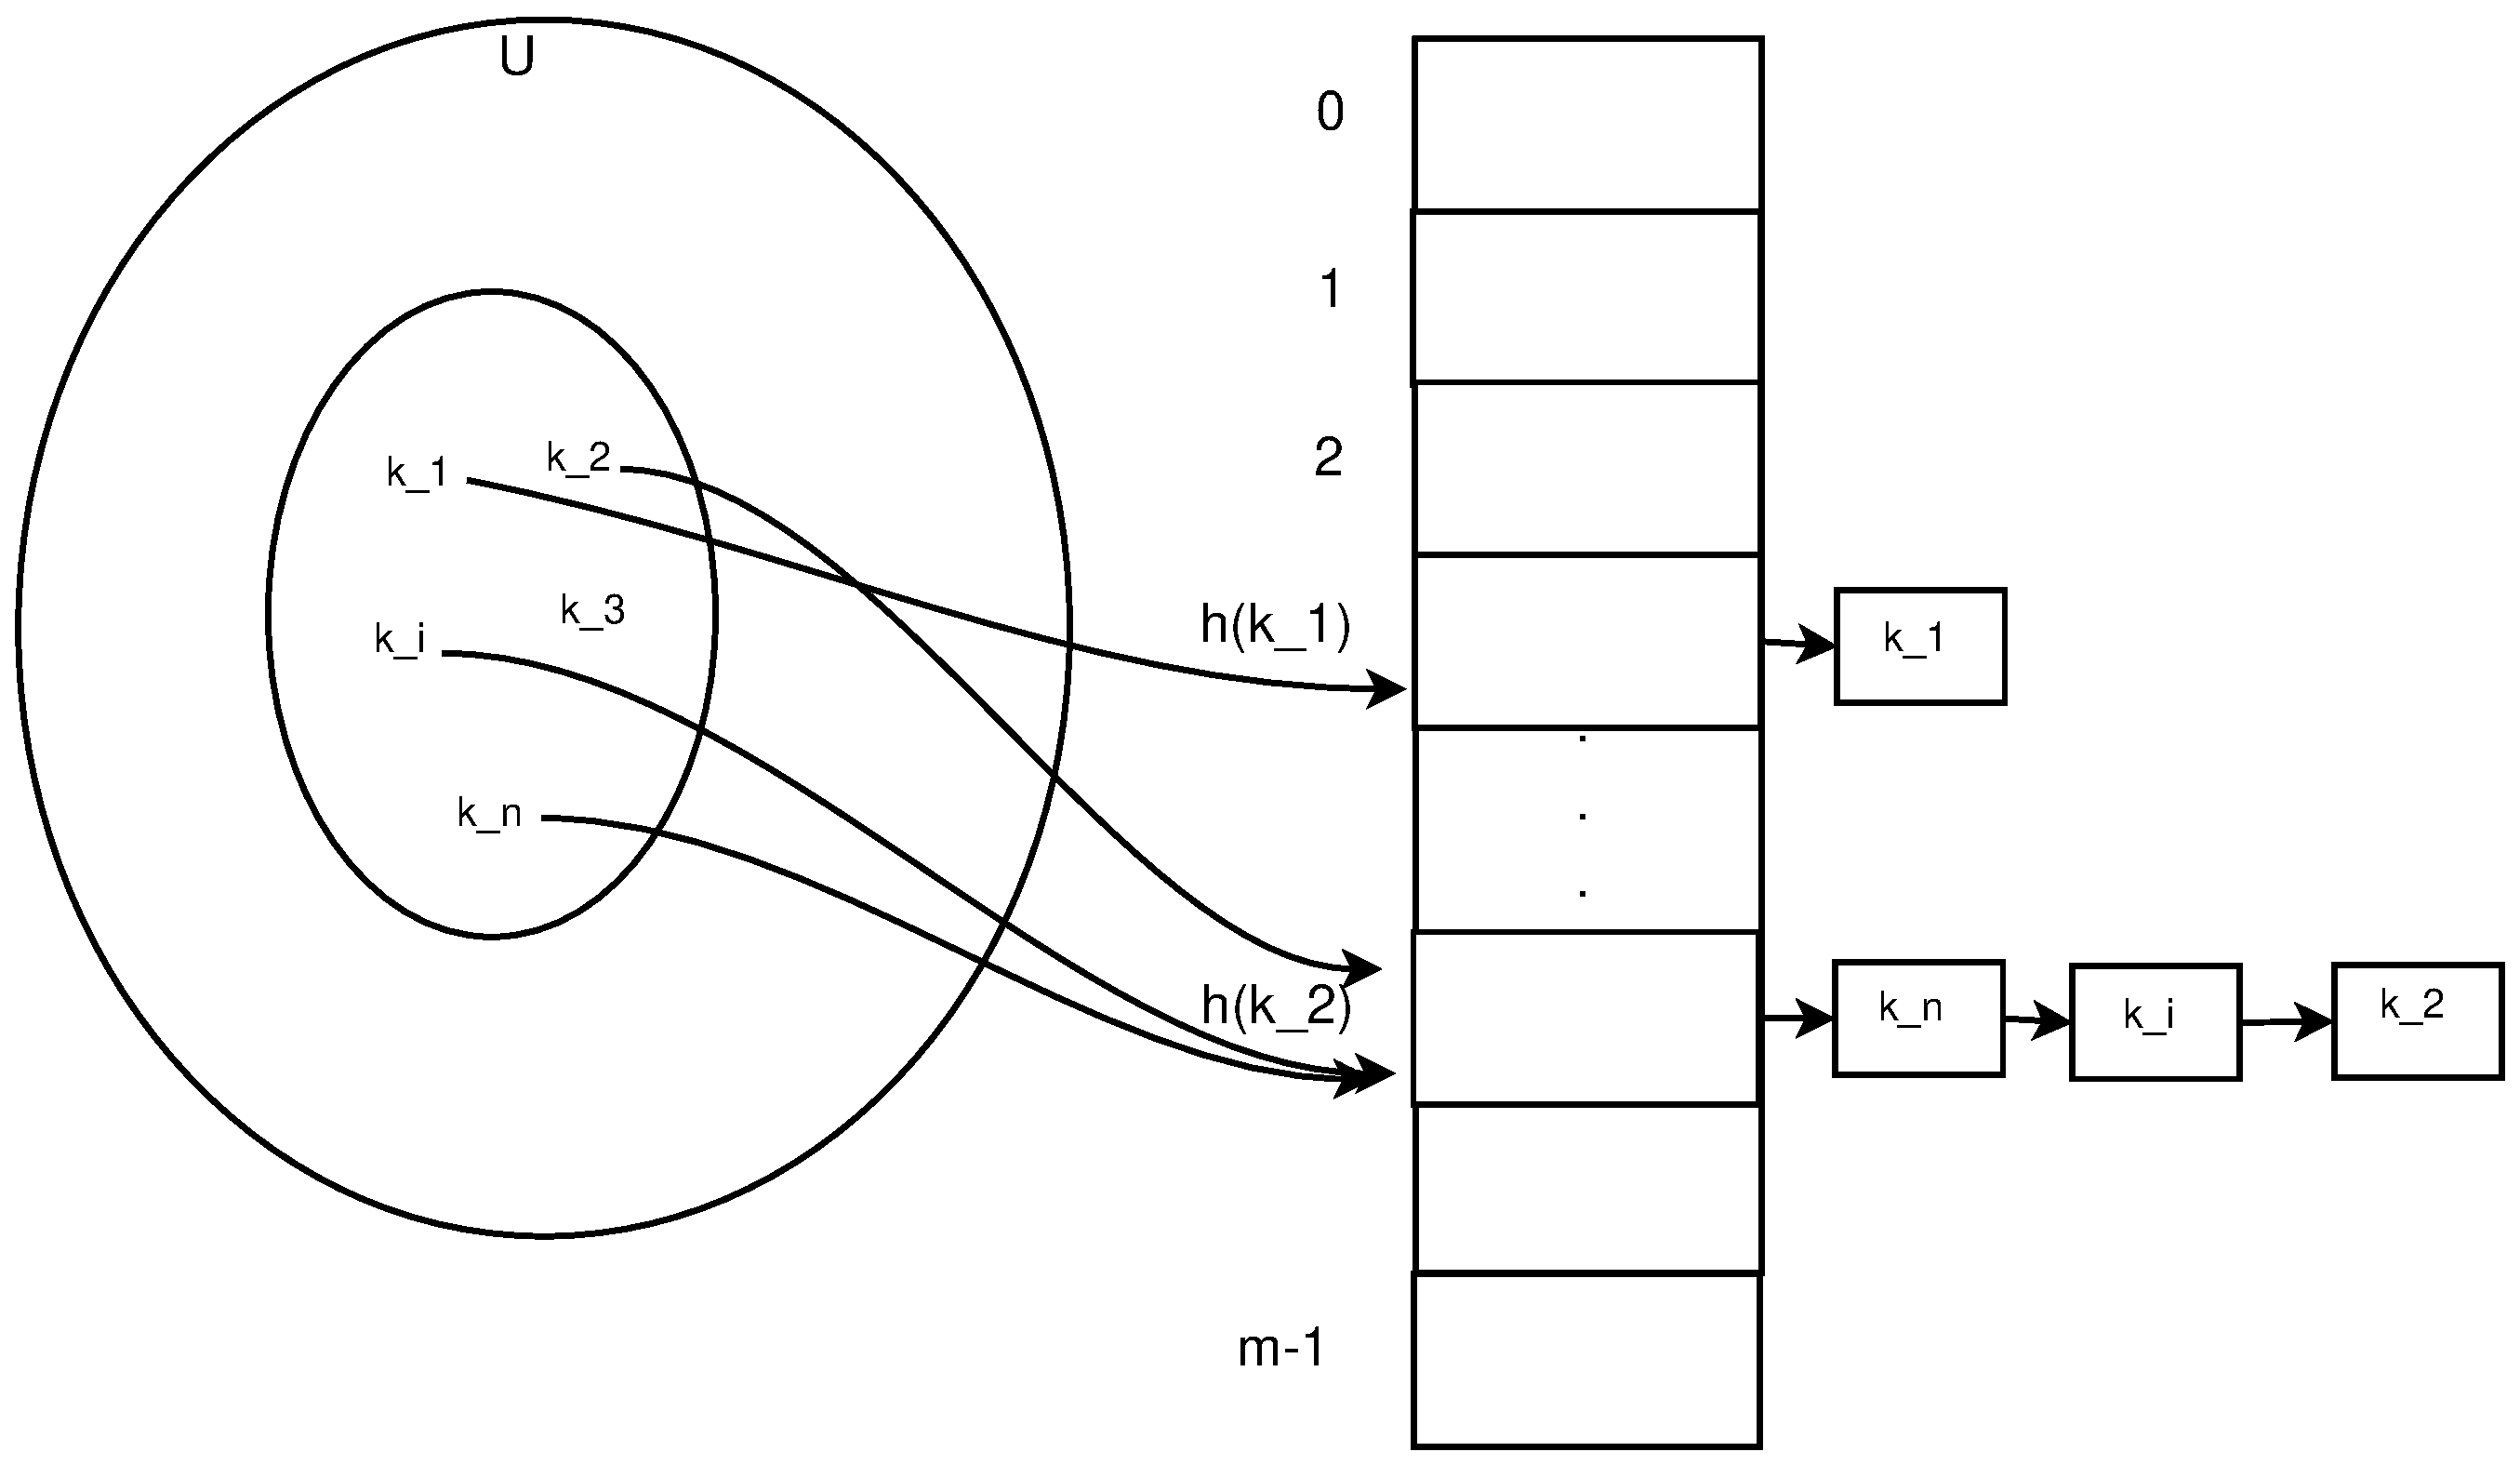
\includegraphics[width=0.8\linewidth]{13/Grafik/hashing}
\end{figure}
$U \subseteq \mathbb{N}$ z.B. 64-Bit-Integer\\
$n=$ Zahl dr zu verwaltenden Schlüssel\\
\[|U| >> n\]
Hashfunktion h:
\[h: U\rightarrow[0,\ldots,m-1]\]
\[\text{z.B. }k\mapsto k \mod m \]
Einfache Annahme: (einfaches uniformes Hashing)
\[\forall~k_i,k_j \in U : Pr(h(k_i)=h(k_j))=\frac{1}{m}   \]
\subsubsection{Analyse der Laufzeit zum Einfügen eines neuen Elementes k}
\begin{itemize}
	\item $h(k)$ berechnen $\longrightarrow O(1)$
	\item Einfügen am Listenanfang in Fach $h(k)$. $\longrightarrow O(1)$
\end{itemize}
\subsubsection{Analyse der Suchzeit für einen Schlüssel $k$}
\begin{itemize}
	\item $h(k)$ $\longrightarrow O(1)$
	\item Listenlänge zum Fach $h(k)$ sei $n_{h(k)}$ also beim Durchlauf der kompletten Liste $\longrightarrow O(n_{h(k)})$
\end{itemize}
\[ E(n_{h(k)})=\frac{n}{m}=\alpha\footnote{Belegungsfaktor} \]
\[ \text{Suchzeit}(\text{Einfügen})\in O(1+\alpha) \]
\subsubsection{Laufzeit beim Löschen von Schlüssel $k$}
\begin{itemize}
	\item $h(k) \longrightarrow O(1)$
	\item Durchlaufen der Liste $\longrightarrow 0(n_{h(k)})$
	\item Löschen durch "`Pointer-Umbiegen"' $\longrightarrow O(1)$
\end{itemize}
\subsection{Universelles Hashing}
\paragraph*{Idee} Arbeite nicht mit einer festen Hashfunktion sondern wähle am Anfang eine zufällige Hashfunktion aus einer Klasse von Hashfunktionen aus.
\paragraph*{z.B.} \[ h_{a,b}(k)=((a\cdot k +b) mod p) mod m \]
p sei eine hinreichend große Primzahl$~~~~0<a<p, 0\leq b < p$
\[ \mathcal{H}_{p,m}=\{ h_{a,b}(k) | 0 < a < p, ~ 0 \leq b < p \} \]
\[ |\mathcal{H}_{p,m}| = p(p-1) \]
\paragraph*{Definition} $\mathcal{H}$ heißt universell $\Leftrightarrow~~\forall~k,l\in U:~ Pr(h(k)=h(l))\leq \frac{1}{m}$
\paragraph*{Suchzeit}
\[ \mathcal{X}_{k,l}=\begin{cases}1&\text{für }h(k)=h(l)\\0&\text{sonst}\end{cases} \]
\[ E(n_{h(k)})=E\left( \sum_{l \in T, l \neq k} \right) =  \sum_{l \in T, l \neq k} E(X_{k,l}) =  \sum_{l \in T, l \neq k} Pr(h(k)=h(l)) = \sum_{l \in T, l \neq k} \frac{1}{m} = \frac{n-1}{m} = \alpha \] 